\documentclass[usenames,dvipsnames,10pt,aspectratio=169]{beamer} 

\usepackage[utf8]{inputenc}
\usepackage{verbatim}
\usepackage{minted}
\usepackage{graphicx}
\usepackage{wrapfig}
\usepackage{geometry}
\usepackage{listings}
% \usepackage{showframe}
\usepackage{enumitem}
\usepackage{color, xcolor}
\usepackage[document]{ragged2e}
\usetheme{umu}

\usemintedstyle{monokai}

\usepackage{hyperref}
\hypersetup{
    colorlinks=true,
    linkcolor=ucugreyish,
    filecolor=ucured,
    urlcolor=ucublue,
}
\urlstyle{same}

%%% Some useful commands
% pdf-friendly newline in links
\newcommand{\pdfnewline}{\texorpdfstring{\newline}{ }} 
% Fill the vertical space in a slide (to put text at the bottom)
\newcommand{\framefill}{\vskip 0pt plus 1 filll}

%%% Enter additional packages below (or above, I can't stop you)! / Jesper
\renewcommand{\proofname}{\sffamily{Proof}}

% custom fullpage image:
% { % all template changes are local to this group.
%     \setbeamertemplate{navigation symbols}{}
%     \begin{frame}<article:0>[plain]
%         \begin{tikzpicture}[remember picture,overlay]
%             \node[at=(current page.center)] {
%                 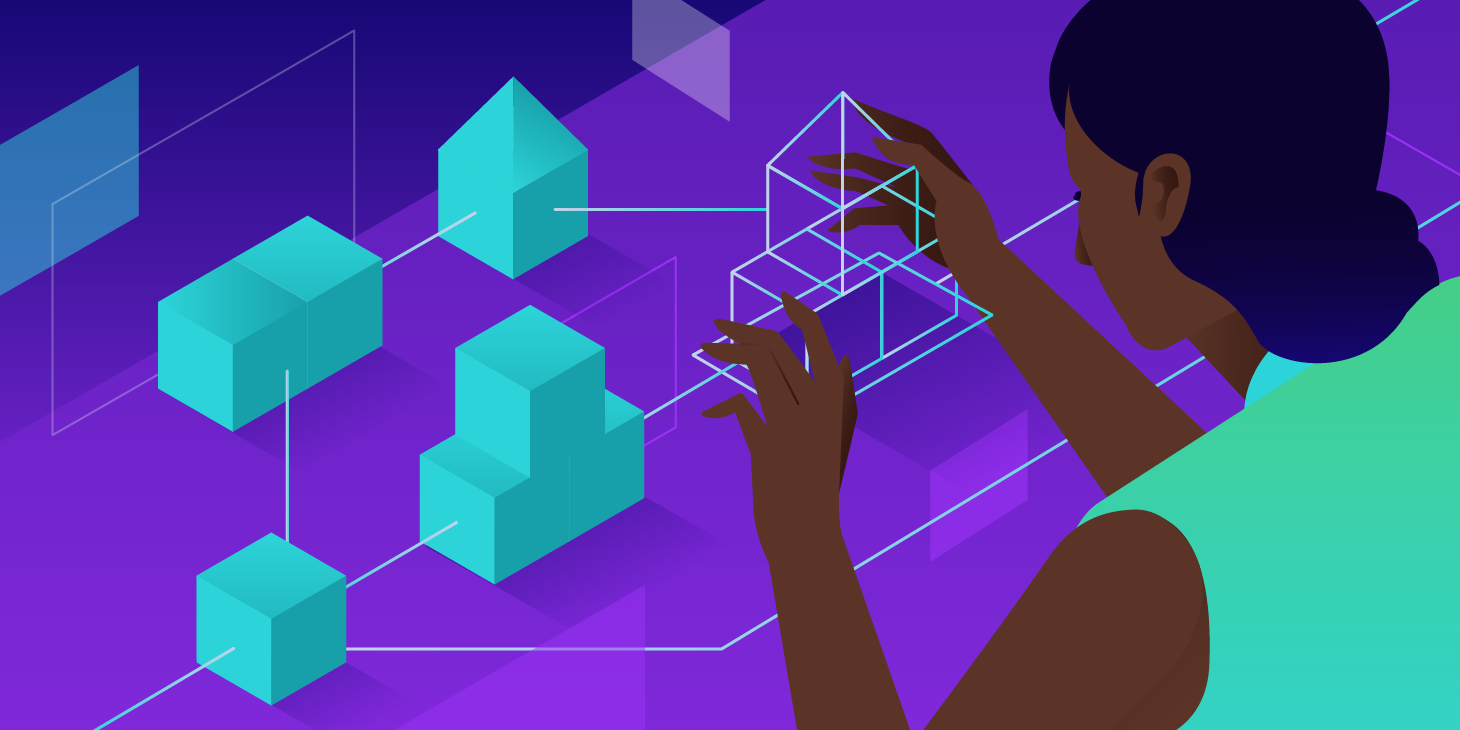
\includegraphics[width=\paperwidth,height=\paperheight]{graphics/version-control.png}
%             };
%         \end{tikzpicture}
%      \end{frame}
% }

% custom shell example inplace
% [fragile] frame
% \begin{lstlisting}[language=Bash, style=shellstyle] 
%     username $ echo a
% \end{lstlisting}

% custom code file
% [fragile] frame
% \lstinputlisting[language=Python, style=codestyle]{code/shebang_ex.py}

% presentation template slides usage
% \framecard[color (not working)]{textbuf}
% \framesplit{Header}{picture}{textbuf}
% \framepic{image}{text}
% \lstinputlisting[language=Bash, style=codestyle]{code/namespace_ex.sh}

%%%%%%%%%%%%%%%%%%%%%%%%%%%%%%%%%%%%%%%%%%%%%%%%%%%%%%%%%%%%%%%%%%%%%%%%%%%%%%%%%%%%%
\title{Linux course}
\subtitle{Bootloaders. Partition tables}
\date[\today]{\small\today}
\author[Morhunenko Mykola]{Morhunenko Mykola}
\institute{APPS@UCU}

\setlist[itemize, 1]{label=$\color{ucublue} \bullet$, leftmargin=-2mm}

\begin{document}

\begin{frame}
\titlepage
\end{frame}

\begin{frame}{Introduction}
    \begin{itemize}
        \item Next two topics are interconnected, and they also are important for understading how to manage the operating system
        \item Important terms:
        \begin{itemize}
            \item \ex{CMOS - Complementary Metal Oxide Semiconductor}. Chip stores the settings like date and time, fan speed, booting sequence
            \item \ex{BIOS - Basic Input/Output System}. Firmware to boot the computer
            \item \ex{UEFI - Unified Extensible Firmware Interface}. Bootloader
            \item \ex{GRUB - GRand Unified Bootloader}. Bootloader
            \item \ex{ESP - EFI System Partition}
            \item \ex{GUID - Globally Unique Identifier (or UUID)}
            \item \ex{MBR - Master Boot Record}. Partition table
            \item \ex{GPT - GUID Partition Table}. Partition table 
        \end{itemize}
    \end{itemize}
\end{frame}

\begin{frame}{\contentsname}
    \setbeamercolor{background canvas}{bg=ucugrey}
    \tableofcontents
\end{frame}

\section{General knowlage}
\framepic{graphics/hardware.jpeg}{\ex[white]{\Huge \textbf{Computer boting procedure}}}
% image source - https://www.wallpaperflare.com/search?wallpaper=semiconductors

\begin{frame}{Boot procedure}
    \begin{itemize}
        \item It will be a very high-level overview of the boot process. For more precise, see \ex{Operating systems} course.
        \item User pressing the button, completing the electronic circuit, and providing the power to all.
        \item The CPU starts up but needs some instructions to work on (remember, the CPU always needs to do something). Since the main memory is empty at this stage, CPU defers to load instructions from the firmware chip on the motherboard and begins executing instructions
        \item The firmware code does a Power On Self Test (POST), initializes the remaining hardware, detects the connected peripherals (mouse, keyboard, pen drive etc.), and checks if all connected devices are healthy. You might remember it as a 'beep' that desktops used to make after POST is successful.
        \item Finally, the firmware code cycles through all storage devices and looks for a bootloader (usually located in the first sector of a disk). If the bootloader is found, then the firmware hands over control of the computer to it.
    \end{itemize}
\end{frame}

\begin{frame}{Boot procedure}
    \begin{itemize}
        \item So now that the bootloader is loaded, its job is to load the rest of the operating system. GRUB is one such bootloader that is capable of loading unix-like operating systems and is also able to chain-load Windows OS. The bootloader is only available in the first sector of a disk, which is 512 bytes. Given the complexity of modern operating systems, some of these bootloaders tend to do multi-stage loading, where the main bootloader loads the second-stage-bootloader in an environment, which is not restricted to 512 bytes.
        \item The bootloader then loads the kernel into memory. Unix-like operating systems then run the init process (the master process, from which other processes are forked/executed) and finally initialize the run-levels.
        \item After all this, and after some other drivers are initialized, the Graphical User Interface (GUI) is loaded, and you are presented with the login screen.
    \end{itemize}
\end{frame}

\framepic{graphics/biosvsefi.png}{}

\framesplit{Bios}{graphics/bios.jpg}{
    \begin{itemize}
        \item \ex{BIOS}is stored on an EPROM (Erasable Programmable Read-Only Memory), allowing the manufacturer to push out updates easily
        \item It provides many helper functions that allow reading boot sectors of attached storage and printing things on screen
        \item \ex{BIOS}menu acces is platform-dependent, but usualy it's pressing \ex{'Del'} or \ex{'F12'} during the initial boot phase
        \item \ex{Intel is not supporting BIOS from 2020}
        \item Uses only \ex{MBR} partitions
    \end{itemize}
}

\framesplit{UEFI}{graphics/uefi.png}{
    \begin{itemize}
        \item \ex{UEFI}does the same job as a BIOS
        \item Stores all data about initialization and startup in an \ex{.efi} file, instead of storing it on the firmware
        \item This .efi file is stored on a special partition called ESP on the hard disk. This ESP partition also contains the bootloader
        \item UEFI supports bigger drive size, provides faster boot time, runs in 32-bit or 64-bit mode, can be used with GPT
        \item Has a \ex{Legacy mode} - UEFI mode that behaves in a way as BIOS did
    \end{itemize}
}

\section{Bootloaders}

{ % all template changes are local to this group.
    \setbeamertemplate{navigation symbols}{}
    \begin{frame}<article:0>[plain]
        \begin{tikzpicture}[remember picture,overlay]
            \node[at=(current page.center)] {
                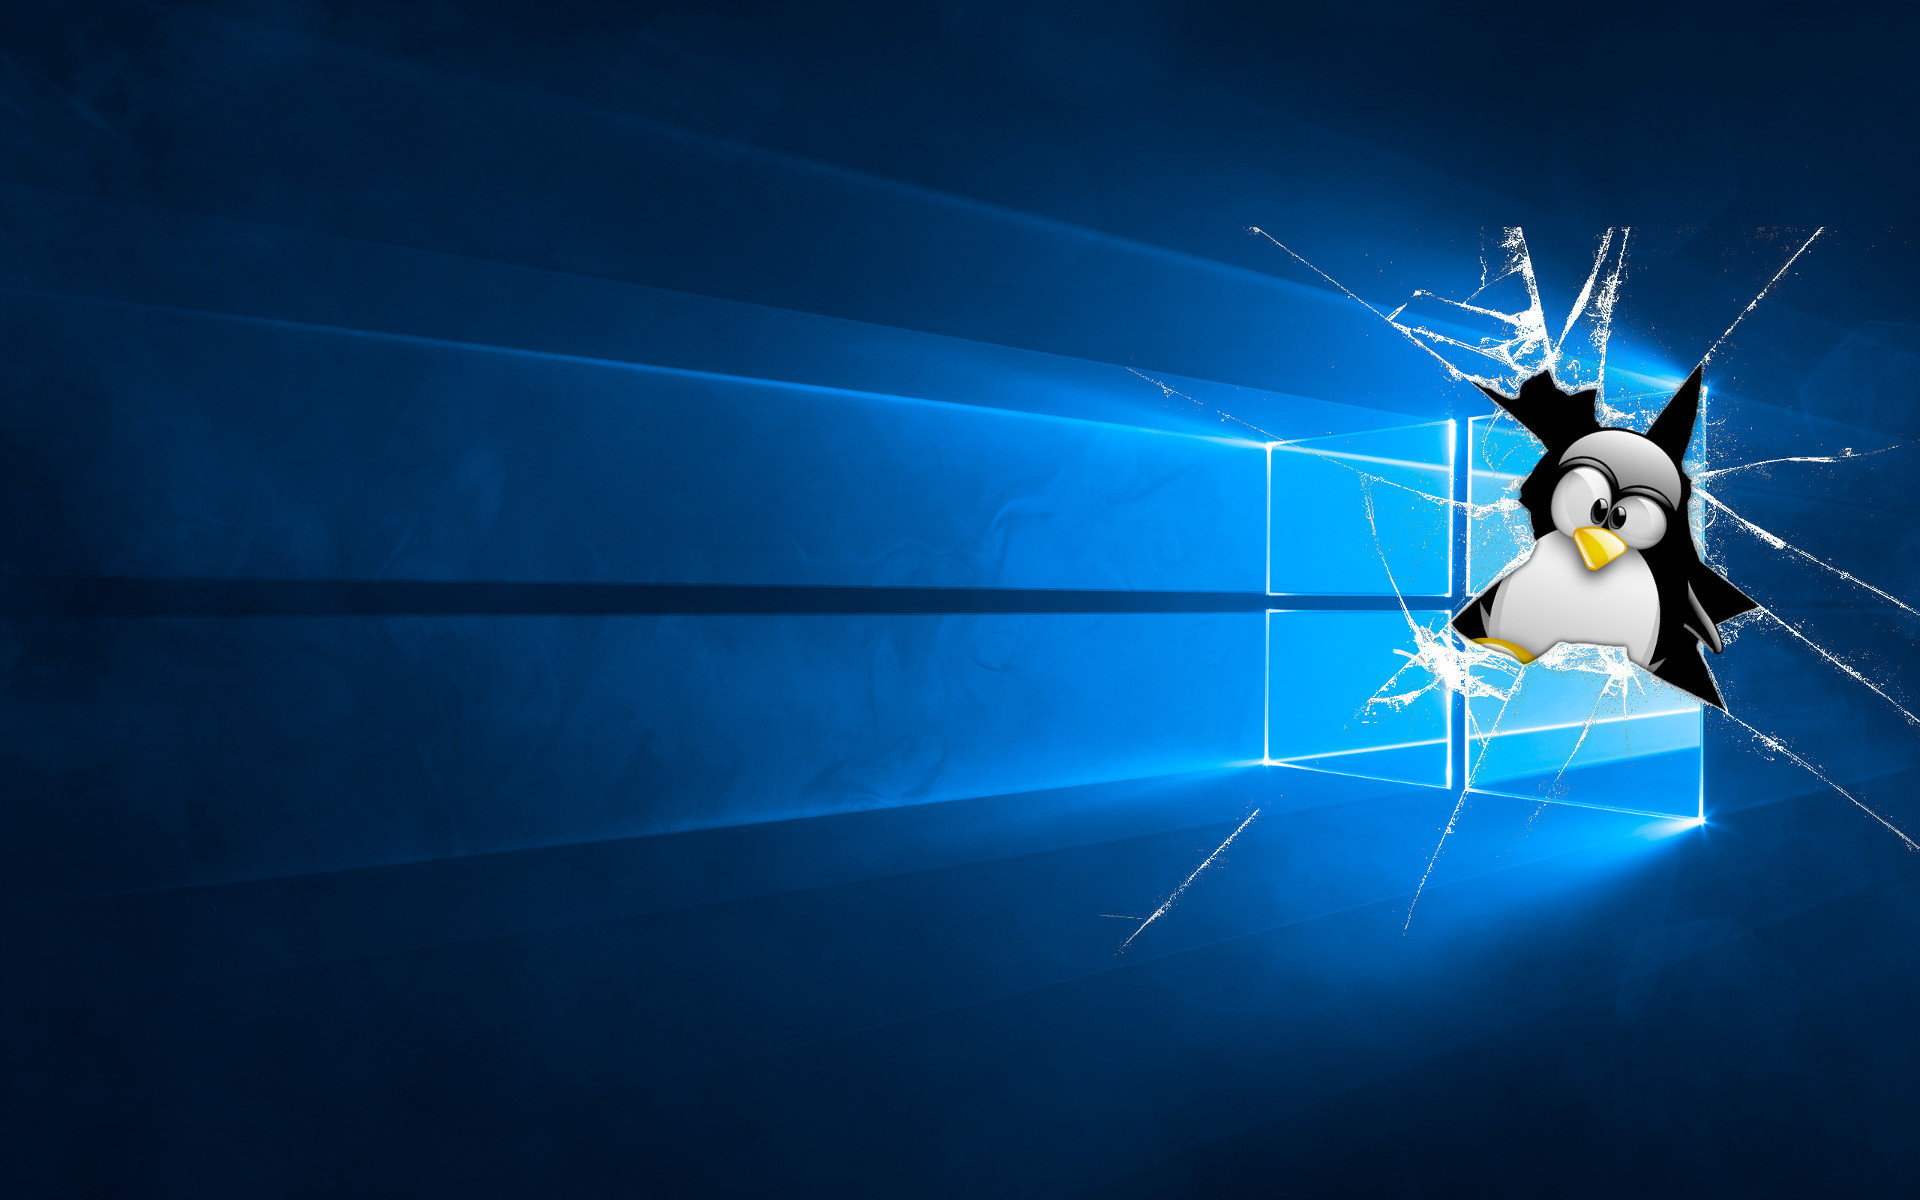
\includegraphics[width=\paperwidth,height=\paperheight]{graphics/boot.jpg}
            };
        \end{tikzpicture}
        {\huge \textbf{Bootloaders}}
     \end{frame}
}

\begin{frame}{Bootloaders overview}
    \begin{itemize}
        \item \ex{Bootloader}- a program responsible for booting the operating system
        \item Bootloader stored on a specific partition
        \item When PC is powered off, all data is stored on the non-volatile memory
        \item But for OS to work, it should be in the RAM
        \item Bootloader is responsible for loading the system to RAM
        \item There are too many platforms and too many ways how bootloaders could be used
        \item To simplify, here is an overview of: x86 architecture, modern Linux OS (kernel v5+)
    \end{itemize}
\end{frame}


\framesplit{GRUB}{graphics/grub.png}{
    \begin{itemize}
        \item GRUB - most wide-common used bootloader for our systems from the GNU project
        \item Can be used in both\ex{UEFI}and\ex{Legacy} modes
        \item If installed, during booting GRUB loads\ex{/boot/grub/grub.cfg}file. Do not edit it!
        \item To change anything in that file, change it only in\ex{/etc/default/grub} \ex[ucuorange]{(remember, there are all setting files)}and then use command \ex{gtub-mkconfig -o /boot/grub/grub.cfg}
        \item But\ex{GRUB} is too old and slow. 
        \item More about it is on \href{https://wiki.archlinux.org/title/GRUB}{Arch wiki}
    \end{itemize}
}

\begin{frame}{systemd-boot}
    \begin{itemize}
        \item Simple UEFI boot manager
        \item Executes configured EFI images
        \item Included with\ex{systemd}
        \item Can only start EFI executables such as UEFI Shell,\ex{Linux \href{https://wiki.archlinux.org/title/EFISTUB}{EFISTAB}}, Windows, GRUB, Windows boot manager etc
        \item Can be installed only with ESP mounted
        \item Much faster than all other bootloaders (\ex{if your init system is systemd}) which is true for both Manjaro and Arch (Ubuntu also)
        \item The reason - it starts fewer things in general and starts almost everything in parallel
        \item Simple in maintaining and setting up:
        \item \ex{bootctl install} for installation
        \item \ex{/boot/loader/entries/} is a location for config files. If you want to add new entry, just add new\ex{.conf}file here
    \end{itemize}
\end{frame}

\section{Partition tables}
\framepic{graphics/devices.jpg}{\vspace{5cm}\hspace{3.5cm}PARTITION TABLES}

\framesplit{Partitioning}{graphics/cfdisk.png}{
    \begin{itemize}
        \item Linux see each device as a separate file a.e.\ex{/dev/sdX, /dev/nvme0nX}
        \item \ex{Partitioning}- adding logical devices remaining the same amount of phisical. It make possible to manage each partition separate
        \item Each such logical device called\ex{partition}
        \item \ex{Partition table}- area on a disk where the disk stores the information about every partition
        \item \ex{Partition editors}can be used to add/delete, adit new partitions (a.e. fdisk, cfdisk, parted, gparted)
    \end{itemize}
}

\framesplit{Master boot record}{graphics/MBR.png}{
    What everybody should know about \ex{MBR}?
    \begin{itemize}
        \item Very old, unfortunately still not deprecated, and you can see it even on the very new laptops
        \item Don't support UEFI
        \item Max disk size - 2TB. If you have more, only 2TB will be visible
        \item Only four general partitions available
        \item \ex[ucured]{Do not use it, use GPT!}
        \item The best and easiest way - delete or move everything from the physical disk and change the partition table
        \item Otherwise - there are some applications for Windows/Linux how to make it without dataloss (usually quite expensive)
    \end{itemize}
}
\begin{frame}{GUID Partition Table} 
        

    {
        
        \begin{columns}[t, totalwidth=\textwidth]
        \begin{column}{0.47\linewidth}
            \begin{center}
                What about \ex{GPT}?
                \begin{itemize}
                    \item \ex{GPT} - also quite old - 30 years - but conceptually still the best way for partitioning
                    \item Can support UEFI
                    \item 128 partitions available
                    \item Max disk size - 18EB. As far as the biggest HDD's I know are only 18TB each it won't be a limitation for nearest decades
                \end{itemize}    
            \end{center}
        \end{column}

        \begin{column}{0.47\linewidth}
            \begin{center}
                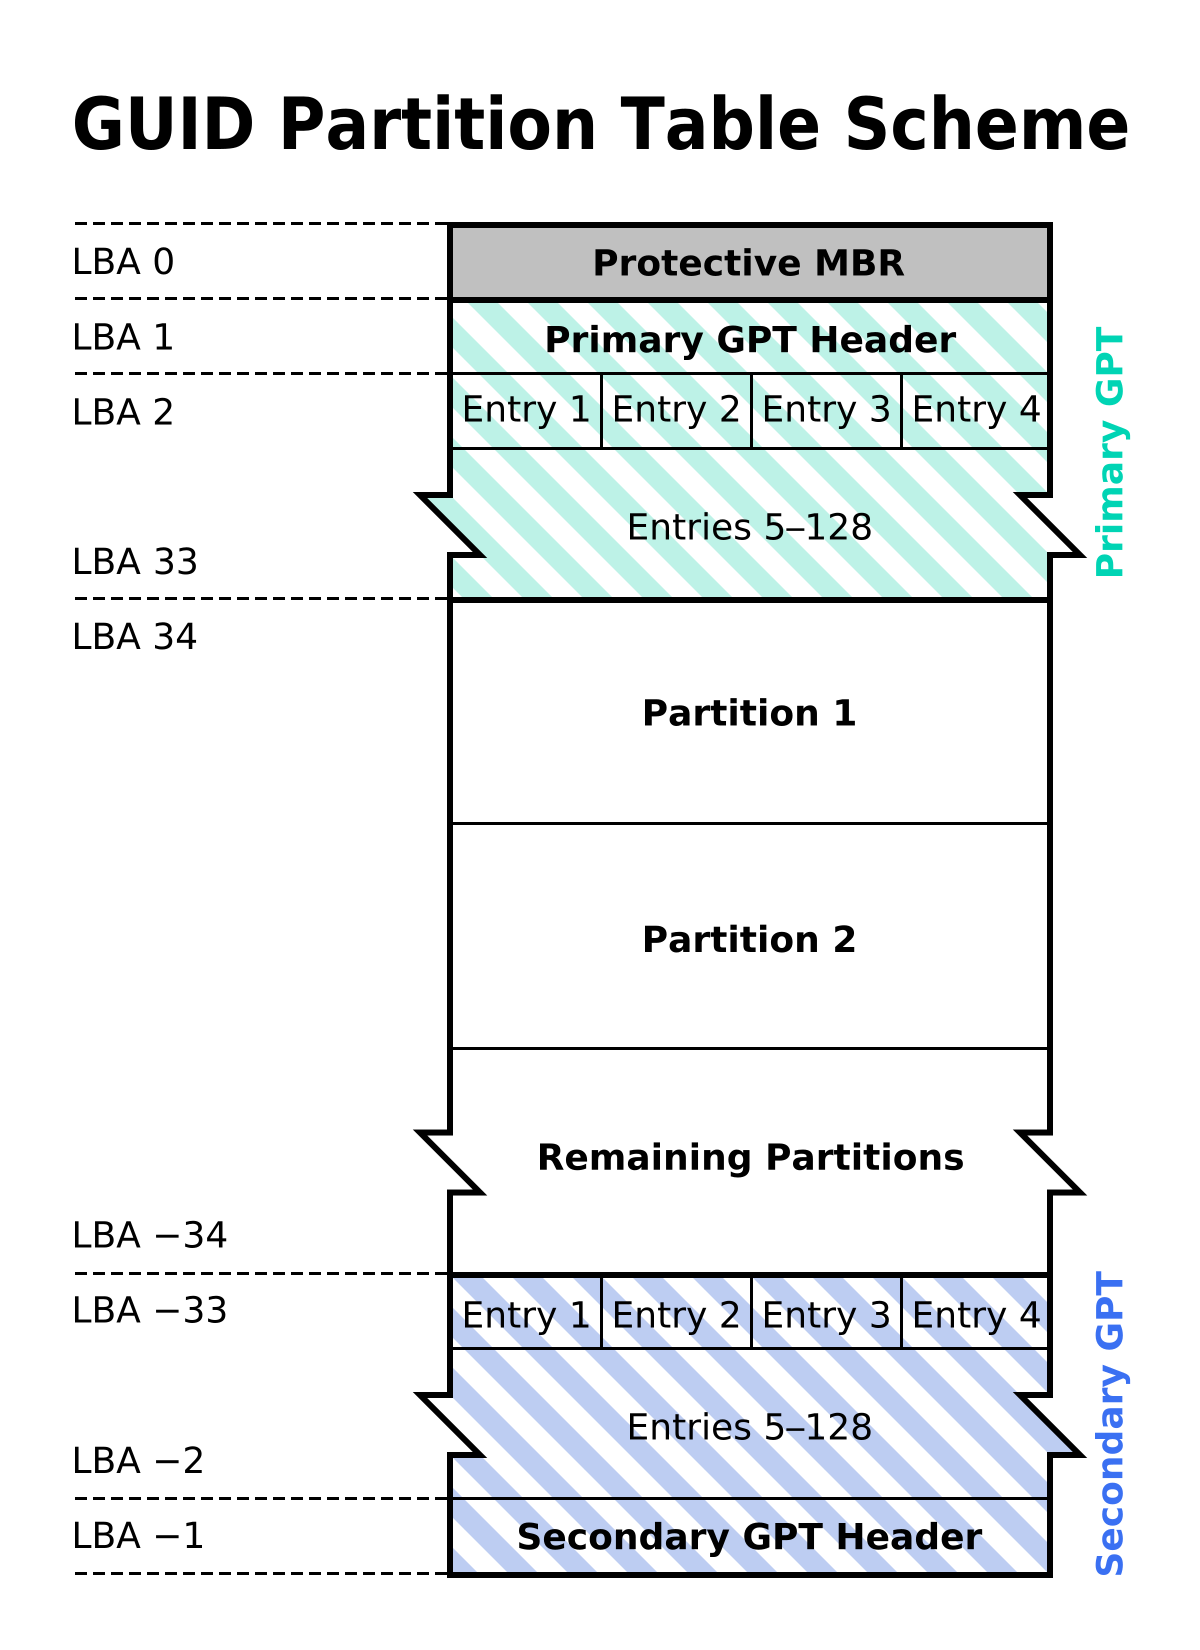
\includegraphics[width=0.8\textwidth]{graphics/GPT.png}    
            \end{center}
        \end{column}

    \end{columns}
    }

\end{frame}

\framesplit{How and why to use partitioning?}{graphics/storage_disk_partitions.png}{
    \begin{itemize}
        \item Usually partitioning is used only when installing a new OS or changing partitions info (add/remove swap, etc)
        \item Usually\ex{cfdisk}is used for such manipulations
        \item For more deep things (create, change, remove table)\ex{parted, Gparted, fdisk}are recommended
        \item 
    \end{itemize}
}


\section{Sources}
\framecard{Sources}
\begin{frame}{Sources}
    \begin{itemize}
        \item UCU Linux Club resources
        \item \href{https://www.freecodecamp.org/news/uefi-vs-bios/}{Boot procedure}
        \item \href{https://en.wikipedia.org/wiki/Bootloader}{Wiki Bootloader}
        \item \href{https://wiki.archlinux.org/title/GRUB}{GRUB Arch Wiki}
        \item \href{https://wiki.archlinux.org/title/Systemd-boot}{Systemd-boot Arch wiki}
        \item \href{https://www.maketecheasier.com/grub-vs-systemd-boot/}{GRUB vs systemd-boot}
        \item \href{https://wiki.archlinux.org/title/Partitioning}{Partitioning Arch wiki}
    \end{itemize}
\end{frame}

\end{document}